%%%% Paramétrage du TD %%%%
\def\xxnumchapitre{Chapitre 0 \vspace{.2cm}}
\def\xxchapitre{\hspace{.12cm} Prise en main de Python}

\def\xxcompetences{%
\textsl{%
\textbf{Savoirs et compétences :}\\
\vspace{-.4cm}
\begin{itemize}[label=\ding{112},font=\color{bleuxp}] 
\item .
%\item \textit{Mod3.C2 : } pôles dominants et réduction de l’ordre du modèle : principe, justification
%\item \textit{Res2.C4 : } stabilité des SLCI : définition entrée bornée -- sortie bornée (EB -- SB)	
%\item \textit{Res2.C5 : } stabilité des SLCI : équation caractéristique	
%\item \textit{Res2.C6 : } stabilité des SLCI : position des pôles dans le plan complexe
%\item \textit{Res2.C7 : } stabilité des SLCI : marges de stabilité (de gain et de phase)
\end{itemize}
}}


\def\xxfigures{
%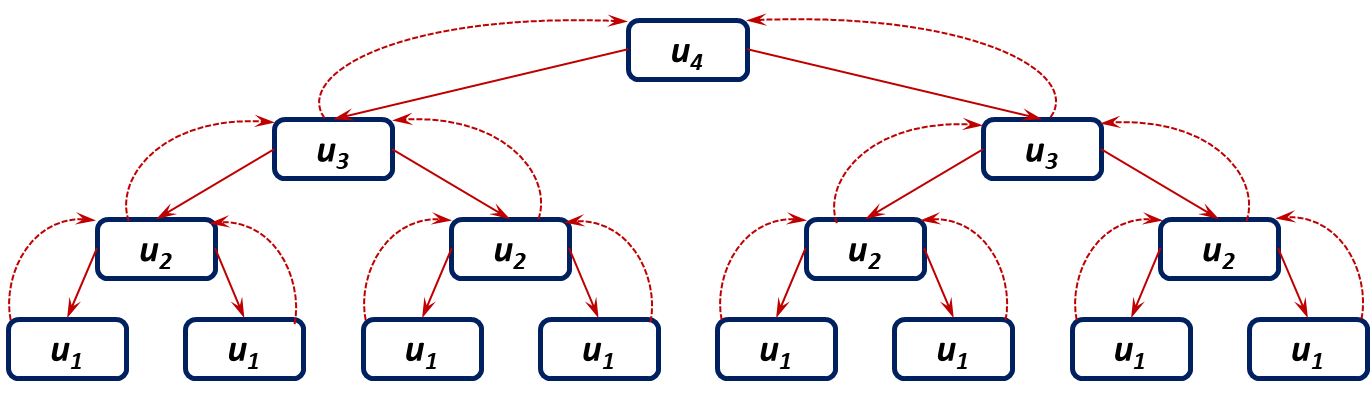
\includegraphics[width=3cm]{fig_01}\\
%\textit{}
}%figues de la page de garde

\def\xxtitreexo{Applications -- Bases}
\def\xxsourceexo{}
\def\xxactivite{{ Application 03} \ifprof  -- Corrigé \else \fi}

%\iflivret
\input{\repRel/Style/pagegarde_TD}
%\else
%\pagestyle{empty}


%%%%%%%% PAGE DE GARDE COURS
\ifcours
\begin{tikzpicture}[remember picture,overlay]
\node at (current page.north west)
{\begin{tikzpicture}[remember picture,overlay]
\node[anchor=north west,inner sep=0pt] at (0,0) {\includegraphics[width=\paperwidth]{\thechapterimage}};
\draw[anchor=west] (-2cm,-8cm) node [line width=2pt,rounded corners=15pt,draw=ocre,fill=white,fill opacity=0.6,inner sep=40pt]{\strut\makebox[22cm]{}};
\draw[anchor=west] (1cm,-8cm) node {\huge\sffamily\bfseries\color{black} %
\begin{minipage}{1cm}
\rotatebox{90}{\LARGE\sffamily\textsc{\color{ocre}\textbf{\xxnumpartie}}}
\end{minipage} \hfill
\begin{minipage}[c]{14cm}
\begin{titrepartie}
\begin{flushright}
\renewcommand{\baselinestretch}{1.1} 
\Large\sffamily\textsc{\textbf{\xxpartie}}
\renewcommand{\baselinestretch}{1} 
\end{flushright}
\end{titrepartie}
\end{minipage} \hfill
\begin{minipage}[c]{3.5cm}
{\large\sffamily\textsc{\textbf{\color{ocre} \discipline}}}
\end{minipage} 
 };
\end{tikzpicture}};
\end{tikzpicture}


\begin{tikzpicture}[overlay]
\node[shape=rectangle, 
      rounded corners = .25 cm,
	  draw= ocre,
	  line width=2pt, 
	  fill = ocre!10,
	  minimum width  = 2.5cm,
	  minimum height = 3cm,] at (18cm,0) {};
\node at (17.7cm,0) {\rotatebox{90}{\textbf{\Large\color{ocre}{\classe}}}};
%{};
\end{tikzpicture}

\vspace{3.5cm}

\begin{tikzpicture}[remember picture,overlay]
\draw[anchor=west] (-2cm,-6cm) node {\huge\sffamily\bfseries\color{black} %
\begin{minipage}{2cm}
\begin{center}
\LARGE\sffamily\textsc{\color{ocre}\textbf{\xxactivite}}
\end{center}
\end{minipage} \hfill
\begin{minipage}[c]{15cm}
\begin{titrechapitre}
\renewcommand{\baselinestretch}{1.1} 
\Large\sffamily\textsc{\textbf{\xxnumchapitre}}

\Large\sffamily\textsc{\textbf{\xxchapitre}}
\vspace{.5cm}

\renewcommand{\baselinestretch}{1} 
\normalsize\normalfont
\xxcompetences
\end{titrechapitre}
\end{minipage}  };
\end{tikzpicture}
\vfill

\begin{flushright}
\begin{minipage}[c]{.3\linewidth}
\begin{center}
\xxfigures
\end{center}
\end{minipage}\hfill
\begin{minipage}[c]{.6\linewidth}
\startcontents
\printcontents{}{1}{}
\end{minipage}
\end{flushright}

\begin{tikzpicture}[remember picture,overlay]
\draw[anchor=west] (4.5cm,-.7cm) node {
\begin{minipage}[c]{.2\linewidth}
\begin{flushright}

\includegraphics[width=2cm]{png/logoCC}
\end{flushright}
\end{minipage}
\begin{minipage}[c]{.2\linewidth}
\textsl{\xxauteur} \\
\textsl{\classe}
\end{minipage}
 };
\end{tikzpicture}
\newpage
\pagestyle{fancy}

\newpage
\pagestyle{fancy}

\else
\fi


%%%%%%%% PAGE DE GARDE TD
\iftd
%\begin{tikzpicture}[remember picture,overlay]
%\node at (current page.north west)
%{\begin{tikzpicture}[remember picture,overlay]
%\draw[anchor=west] (-2cm,-3.25cm) node [line width=2pt,rounded corners=15pt,draw=ocre,fill=white,fill opacity=0.6,inner sep=40pt]{\strut\makebox[22cm]{}};
%\draw[anchor=west] (1cm,-3.25cm) node {\huge\sffamily\bfseries\color{black} %
%\begin{minipage}{1cm}
%\rotatebox{90}{\LARGE\sffamily\textsc{\color{ocre}\textbf{\xxnumpartie}}}
%\end{minipage} \hfill
%\begin{minipage}[c]{13.5cm}
%\begin{titrepartie}
%\begin{flushright}
%\renewcommand{\baselinestretch}{1.1} 
%\Large\sffamily\textsc{\textbf{\xxpartie}}
%\renewcommand{\baselinestretch}{1} 
%\end{flushright}
%\end{titrepartie}
%\end{minipage} \hfill
%\begin{minipage}[c]{3.5cm}
%{\large\sffamily\textsc{\textbf{\color{ocre} \discipline}}}
%\end{minipage} 
% };
%\end{tikzpicture}};
%\end{tikzpicture}

%%%%%%%%%% PAGE DE GARDE TD %%%%%%%%%%%%%%%
%\begin{tikzpicture}[overlay]
%\node[shape=rectangle, 
%      rounded corners = .25 cm,
%	  draw= ocre,
%	  line width=2pt, 
%	  fill = ocre!10,
%	  minimum width  = 2.5cm,
%	  minimum height = 2.5cm,] at (18.5cm,0) {};
%\node at (17.7cm,0) {\rotatebox{90}{\textbf{\Large\color{ocre}{\classe}}}};
%%{};
%\end{tikzpicture}

% PARTIE ET CHAPITRE
%\begin{tikzpicture}[remember picture,overlay]
%\draw[anchor=west] (-1cm,-2.1cm) node {\large\sffamily\bfseries\color{black} %
%\begin{minipage}[c]{15cm}
%\begin{flushleft}
%\xxnumchapitre \\
%\xxchapitre
%\end{flushleft}
%\end{minipage}  };
%\end{tikzpicture}

% Bandeau titre exo
\begin{tikzpicture}[remember picture,overlay]
\draw[anchor=west] (-2cm,-4cm) node {\huge\sffamily\bfseries\color{black} %
\begin{minipage}{5cm}
\begin{center}
\LARGE\sffamily\color{ocre}\textbf{\textsc{\xxactivite}}

\begin{center}
\xxfigures
\end{center}

\end{center}
\end{minipage} \hfill
\begin{minipage}[c]{12cm}
\begin{titrechapitre}
\renewcommand{\baselinestretch}{1.1} 
\large\sffamily\textbf{\textsc{\xxtitreexo}}

\small\sffamily{\textbf{\textit{\color{black!70}\xxsourceexo}}}
\vspace{.5cm}

\renewcommand{\baselinestretch}{1} 
\normalsize\normalfont
\xxcompetences
\end{titrechapitre}
\end{minipage}  };
\end{tikzpicture}
\else
\fi


%%%%%%%% PAGE DE GARDE FICHE
\iffiche
\begin{tikzpicture}[remember picture,overlay]
\node at (current page.north west)
{\begin{tikzpicture}[remember picture,overlay]
\draw[anchor=west] (-2cm,-3.25cm) node [line width=2pt,rounded corners=15pt,draw=ocre,fill=white,fill opacity=0.6,inner sep=40pt]{\strut\makebox[22cm]{}};
\draw[anchor=west] (1cm,-3.25cm) node {\huge\sffamily\bfseries\color{black} %
\begin{minipage}{1cm}
\rotatebox{90}{\LARGE\sffamily\textsc{\color{ocre}\textbf{\xxnumpartie}}}
\end{minipage} \hfill
\begin{minipage}[c]{14cm}
\begin{titrepartie}
\begin{flushright}
\renewcommand{\baselinestretch}{1.1} 
\large\sffamily\textsc{\textbf{\xxpartie} \\} 

\vspace{.2cm}

\normalsize\sffamily\textsc{\textbf{\xxnumchapitre -- \xxchapitre}}
\renewcommand{\baselinestretch}{1} 
\end{flushright}
\end{titrepartie}
\end{minipage} \hfill
\begin{minipage}[c]{3.5cm}
{\large\sffamily\textsc{\textbf{\color{ocre} \discipline}}}
\end{minipage} 
 };
\end{tikzpicture}};
\end{tikzpicture}


\begin{tikzpicture}[overlay]
\node[shape=rectangle, 
      rounded corners = .25 cm,
	  draw= ocre,
	  line width=2pt, 
	  fill = ocre!10,
	  minimum width  = 2.5cm,
	  minimum height = 2.5cm,] at (18.5cm,0.5cm) {};
%	  minimum height = 2.5cm,] at (18.5cm,0cm) {};
\node at (17.7cm,0.5) {\rotatebox{90}{\textsf{\textbf{\large\color{ocre}{\classe}}}}};
%{};
\end{tikzpicture}

\else
\fi



%\fi

\setlength{\columnseprule}{.1pt}

\pagestyle{fancy}
\thispagestyle{plain}


\vspace{4.5cm}

\def\columnseprulecolor{\color{bleuxp}}
\setlength{\columnseprule}{0.4pt} 







\ifprof
\vspace{1cm}
\else
\begin{multicols}{2}
\fi



\section*{Les fonctions}
Nous avons déjà rencontré des fonctions python prédéfinies : \texttt{type}, \texttt{int}, \texttt{len}, \texttt{print}... 

%\subsection{Utilisation de l'aide}
Lorsqu'on écrit le nom d'une fonction \texttt{fct} dans l'interpréteur et sa parenthèse ouvrante, des informations s'affichent (les \textbf{arguments} attendus et optionnels, parfois le type du résultat...). \\
Pour obtenir plus de détails, on peut aussi taper \texttt{help(fct)}.

\exer{}

\question{
 \`A l'aide de ces deux techniques : vérifier que la fonction \texttt{abs} renvoie bien la valeur absolue, comprendre le fonctionnement de la fonction \texttt{round}, et tester avec des exemples pour vérifier.}





%\emph{Remarque:} On peut aussi, après avoir tapé \texttt{import math}, consulter l'aide du module \texttt{math} en tapant \texttt{help(math)}. %La commande \texttt{dir(math)} permet de lister toutes les commandes présentes dans ce module.\\ 

%On peut aussi consulter l'aide sur internet  notamment sur \texttt{docs.python.org}, mais il faut savoir trier les informations.


\subsection*{Fonctions issues d'une bibliothèque}
Souvent, nous aurons besoin de fonctions non disponibles par défaut, qu'il faut alors importer à partir d'une bibliothèque\footnote{Remarque : en anglais, bibliothèque se dit \emph{library}.}. C'est le cas pour de nombreuses fonctions mathématiques ; par exemple : 
\begin{lstlisting} 
>>> cos(1)
	Traceback (most recent call last):
	File "<pyshell#27>", line 1, in <module>
 	cos(1)
NameError: name 'cos' is not defined
\end{lstlisting}

%Importons la bibliothèque \texttt{math} ; voici une méthode possible : 
\begin{lstlisting}
>>> import math as m # ceci signifie "importer la bibliothèque math sous le nom m"
>>> m.cos(1)
        0.5403023058681398
\end{lstlisting}



%Quelques fonctions mathématiques usuelles sont dans cette bibliothèque : \\\texttt{cos, sin, tan, exp, log} (logarithme népérien noté $\ln$ en mathématiques), \\\texttt{sqrt} (racine carrée : "\textbf{sq}uare \textbf{r}oo\textbf{t}"), \\
\texttt{floor} (partie entière habituelle : \texttt{floor(x)} est l'entier inférieur le plus proche de \texttt{x}),\\
\texttt{ceil} (partie entière supérieure : \texttt{ceil(x)} est l'entier supérieur le plus proche de \texttt{x}).\\

%Si on a besoin de toutes les fonctions contenues dans une bibliothèque, on peut les importer toutes d'un coup de la manière suivante\footnote{Technique à utiliser avec précaution car des bibliothèques différentes peuvent comporter des fonctions avec le même nom, sans que ces fonctions soient identiques. Si vous faites appel à une fonction présente dans deux bibliothèques importées, vous ne savez pas laquelle vous utilisez vraiment ! } : 
\begin{lstlisting}
>>> from math import *
\end{lstlisting}


\subsection*{Définir vos propres fonctions}
Vous pouvez définir vos propres fonctions. Pour cela il faut se placer dans le script TP0.py et plus dans le shell. Une fonction se définit de la façon suivante:

\begin{lstlisting}
def f(x): # Def appelle une fonction et f indique son nom 
    return(x**2) 
\end{lstlisting}


On dit que la variable \texttt{x} est l'\emph{argument} de la fonction \texttt{f}, et que cette fonction \emph{renvoie} (ou \emph{retourne})   $\mathtt{x^2}$.\\

%Après avoir écrit les \texttt{:}, lors du passage à la ligne, il y a une \textbf{indentation} automatique : elle est indispensable, elle permet à Python de savoir si ce qui fait partie de la définition de la fonction et ce qui n'en fait plus partie. 
C'était la même chose pour la structure \texttt{for}.




%Après avoir défini une fonction, on peut l'évaluer en une valeur précise : par exemple, exécutez le script, et dans le shell, calculez  $f(12)$.\\

%Une fonction n'associe pas forcément un réel à un réel ; par exemple, la fonction suivante renvoie \texttt{True} ou \texttt{False} selon que l'argument entier \texttt{n} est pair ou non : 

\begin{lstlisting}
def g(n):
    return( (n \% 2) == 0 )
\end{lstlisting}


Une fonction peut avoir plusieurs arguments, que l'on sépare alors par des virgules ; le bloc d'instruction peut être plus long : 
\begin{lstlisting}
def h(x,y):
    z = 2 * y
    return(x + z)
\end{lstlisting}

%(On aurait cependant pu se contenter d'une seule instruction : \texttt{return(x + 2 * y)} )\\
La syntaxe générale d'une fonction est la suivante : 
\begin{lstlisting}
def nom_de_la_fonction(arguments):
\end{lstlisting}

%Le chapitre 3 au cours de la séance de TP01 propose des applications qui portent sur l'utilisation de fonctions dans l'algorithme. 

\exer{}

\question{\'Ecrire une fonction \texttt{suite\_cos} qui prend pour argument un entier naturel \texttt{n} et qui affiche toutes les valeurs de $\cos(i)$ pour $i$ variant de $0$ à \texttt{n-1}.}






\ifprof
\else
\end{multicols}
\fi

